\chapter{Preventivo}\label{Preventivo}

In questa sezione il gruppo \textit{Jawa Druids} descrive come userà le risorse a sua disposizione. Per identificarli nelle tabelle, i ruoli vengono indicati con le seguenti sigle:
\begin{itemize}
	\item \textbf{Re}: \textit{Responsabile};
	\item \textbf{Am}: \textit{Amministratore};
	\item \textbf{An}: \textit{Analista};
	\item \textbf{Pt}: \textit{Progettista};
	\item \textbf{Pr}: \textit{Programmatore};
	\item \textbf{Ve}: \textit{Verificatore}.
\end{itemize}
\clearpage
\section{Fase di Analisi}\label{PreventivoFaseDiAnalisi}

\subsection{Prospetto orario}\label{PreventivoFaseDiAnalisiProspettoOrario}
In questa fase la distribuzione oraria è la seguente:
\quad
\def\tabularxcolumn#1{m{#1}}
{\rowcolors{2}{RawSienna!90!RawSienna!20}{RawSienna!70!RawSienna!40}

	\begin{center}
		\renewcommand{\arraystretch}{1.4}
		\begin{tabularx}{\textwidth}{|X|c|c|c|c|c|c|c|}
			\hline
			\rowcolor{airforceblue}
			\textbf{Nominativo} & \textbf{Re} & \textbf{Am} & \textbf{An} & \textbf{Pt} & \textbf{Pr} & \textbf{Ve} & \textbf{Totale ore}\\
			\hline
			\textit{Andrea Dorigo} & 10 & 7 & 3 & 0 & 0 & 5 & 25\\
			\hline
			\textit{Margherita Mitillo} & 8 & 3 & 13 & 0 & 0 & 1 & 25\\
			\hline
			\textit{Igli Mezini} & 3 & 6 & 8 & 0 & 0 & 8 & 25\\
			\hline
			\textit{Andrea Cecchin} & 5 & 9 & 9 & 0 & 0 & 2 & 25\\
			\hline
			\textit{Emma Roveroni} & 2 & 5 & 7 & 0 & 0 & 11 & 25\\
			\hline
			\textit{Alfredo Graziano} & 0 & 10 & 9 & 0 & 0 & 6 & 25\\
			\hline
			\textit{Mattia Cocco} & 1 & 9 & 8 & 0 & 0 & 7 & 25\\
			\hline
			Totale ore ruolo & 29 & 49 & 57 & 0 & 0 & 40 & 175\\
			\hline
		\end{tabularx}
	\captionof{table}{\textbf{Distribuzione delle ore durante l'Analisi}}
	\end{center}

Il seguente istogramma riassume i dati ottenuti:
\begin{figure}[!h]
	\begin{center}
		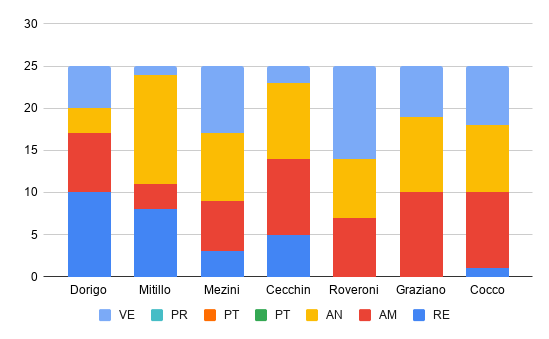
\includegraphics[width=0.7\linewidth]{../immagini/pdp/istogramma_analisi.png}
		\caption{Istogramma della ripartizione oraria durante la Analisi}
	\end{center}
\end{figure}
\clearpage
\subsection{Prospetto economico}\label{PreventivoFaseDiAnalisiProspettoEconomico}
\quad
\def\tabularxcolumn#1{m{#1}}
{\rowcolors{2}{RawSienna!90!RawSienna!20}{RawSienna!70!RawSienna!40}
	\begin{center}
		\renewcommand{\arraystretch}{1.4}
		\begin{tabularx}{7cm}{|X|c|c|}
			\hline
			\rowcolor{airforceblue}
			\textbf{Ruolo} & \textbf{Ore} & \textbf{Costo}\\
			\hline
			Responsabile & 29 & 870\euro\\
			\hline
			Amministratore & 49 & 980\euro\\
			\hline
			Analista & 57 & 1425\euro\\
			\hline
			Progettista & 0 & 0\euro\\
			\hline
			Programmatore & 0 & 0\euro\\
			\hline
			Verificatore & 40 & 600\euro\\
			\hline
			Totale & 175 & 3875\euro\\
			\hline
		\end{tabularx}
	\captionof{table}{\textbf{Prospetto dei costi per ruolo nel periodo di Analisi}}
	\end{center}
Il seguente grafico a torta riassume i dati ottenuti:
\begin{figure}[!ht]
	\begin{center}
		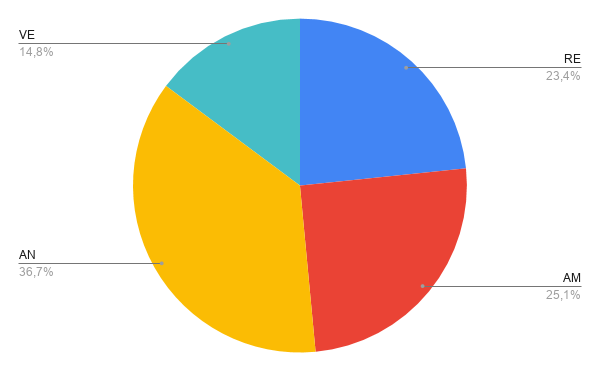
\includegraphics[width=0.8\linewidth]{../immagini/pdp/torta_analisi.png}
		\caption{Grafico a torta della ripartizione per ruolo delle ore nel periodo di Analisi}
	\end{center}
\end{figure}
\clearpage
\section{Fase di Consolidamento dei requisiti}\label{PreventivoFaseDiConsolidamentoDeiRequisiti}

\subsection{Prospetto orario}\label{PreventivoFaseDiConsolidamentoDeiRequisitiProspettoOrario}
In questa fase la distribuzione oraria è la seguente:
\quad
\def\tabularxcolumn#1{m{#1}}
{\rowcolors{2}{RawSienna!90!RawSienna!20}{RawSienna!70!RawSienna!40}

	\begin{center}
		\renewcommand{\arraystretch}{1.4}
		\begin{tabularx}{\textwidth}{|X|c|c|c|c|c|c|c|}
			\hline
			\rowcolor{airforceblue}
			\textbf{Nominativo} & \textbf{Re} & \textbf{Am} & \textbf{An} & \textbf{Pt} & \textbf{Pr} & \textbf{Ve} & \textbf{Totale ore}\\
			\hline
			\textit{Andrea Dorigo} & 0 & 2 & 0 & 0 & 0 & 2 & 4\\
			\hline
			\textit{Margherita Mitillo} & 0 & 2 & 1 & 0 & 0 & 1 & 4\\
			\hline
			\textit{Igli Mezini} & 1 & 1 & 0 & 0 & 0 & 2 & 4\\
			\hline
			\textit{Andrea Cecchin} & 1 & 0 & 2 & 0 & 0 & 1 & 4\\
			\hline
			\textit{Emma Roveroni} & 1 & 1 & 0 & 0 & 0 & 2 & 4\\
			\hline
			\textit{Alfredo Graziano} & 1 & 2 & 1 & 0 & 0 & 0 & 4\\
			\hline
			\textit{Mattia Cocco} & 1 & 0 & 1 & 0 & 0 & 2 & 4\\
			\hline
			Totale ore ruolo & 5 & 8 & 5 & 0 & 0 & 10 & 28\\
			\hline
		\end{tabularx}
	\captionof{table}{\textbf{Distribuzione delle ore durante il Consolidamento dei requisiti}}
	\end{center}
Il seguente istogramma riassume i dati ottenuti:
\begin{figure}[!ht]
	\begin{center}
		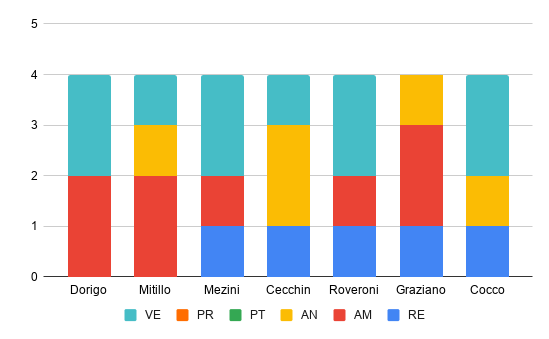
\includegraphics[width=0.7\linewidth]{../immagini/pdp/istogramma_consolidamento_requisiti.png}
		\caption{Istogramma della ripartizione oraria durante il Consolidamento dei requisiti
}
	\end{center}
\end{figure}

\subsection{Prospetto economico}\label{PreventivoFaseDiConsolidamentoDeiRequisitiProspettoEconomico}
\quad
\def\tabularxcolumn#1{m{#1}}
{\rowcolors{2}{RawSienna!90!RawSienna!20}{RawSienna!70!RawSienna!40}
	\begin{center}
		\renewcommand{\arraystretch}{1.4}
		\begin{tabularx}{7cm}{|X|c|c|}
			\hline
			\rowcolor{airforceblue}
			\textbf{Ruolo} & \textbf{Ore} & \textbf{Costo}\\
			\hline
			Responsabile & 5 & 150\euro\\
			\hline
			Amministratore & 8 & 160\euro\\
			\hline
			Analista & 5 & 125\euro\\
			\hline
			Progettista & 0 & 0\euro\\
			\hline
			Programmatore & 0 & 0\euro\\
			\hline
			Verificatore & 10 & 150\euro\\
			\hline
			Totale & 28 & 585\euro\\
			\hline
		\end{tabularx}
	\captionof{table}{\textbf{Prospetto dei costi per ruolo nel periodo di Consolidamento dei requisiti}}
	\end{center}
Il seguente grafico a torta riassume i dati ottenuti:
\begin{figure}[!ht]
	\begin{center}
		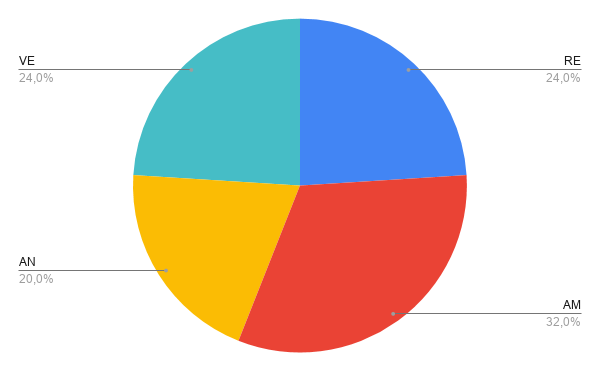
\includegraphics[width=0.8\linewidth]{../immagini/pdp/torta_consolidamento_requisiti.png}
		\caption{Grafico a torta della ripartizione per ruolo delle ore durante il periodo di Consolidamento dei requisiti}
	\end{center}
\end{figure}

\section{Fase di Progettazione architetturale}\label{PreventivoFaseDiProgettazioneArchitetturale}

\subsection{Prospetto orario}\label{PreventivoFaseDiProgettazioneArchitetturaleProspettoOrario}
In questa fase la distribuzione oraria è la seguente:
\quad
\def\tabularxcolumn#1{m{#1}}
{\rowcolors{2}{RawSienna!90!RawSienna!20}{RawSienna!70!RawSienna!40}

	\begin{center}
		\renewcommand{\arraystretch}{1.4}
		\begin{tabularx}{\textwidth}{|X|c|c|c|c|c|c|c|}
			\hline
			\rowcolor{airforceblue}
			\textbf{Nominativo} & \textbf{Re} & \textbf{Am} & \textbf{An} & \textbf{Pt} & \textbf{Pr} & \textbf{Ve} & \textbf{Totale ore}\\
			\hline
			\textit{Andrea Dorigo} & 5 & 3 & 2 & 16 & 4 & 5 & 35\\
			\hline
			\textit{Margherita Mitillo} & 5 & 7 & 2 & 12 & 0 & 9 & 35\\
			\hline
			\textit{Igli Mezini} & 4 & 2 & 8 & 8 & 3 & 10 & 35\\
			\hline
			\textit{Andrea Cecchin} & 7 & 5 & 4 & 10 & 2 & 7 & 35\\
			\hline
			\textit{Emma Roveroni} & 1 & 7 & 4 & 14 & 0 & 9 & 35\\
			\hline
			\textit{Alfredo Graziano} & 2 & 2 & 9 & 15 & 2 & 5 & 35\\
			\hline
			\textit{Mattia Cocco} & 6 & 2 & 6 & 11 & 1 & 9 & 35\\
			\hline
			Totale ore ruolo & 30 & 28 & 35 & 86 & 12 & 54 & 245\\
			\hline
		\end{tabularx}
	\captionof{table}{\textbf{distribuzione delle ore durante la Progettazione architetturale}}
	\end{center}

Il seguente istogramma riassume i dati ottenuti:
\begin{figure}[!h]
	\begin{center}
		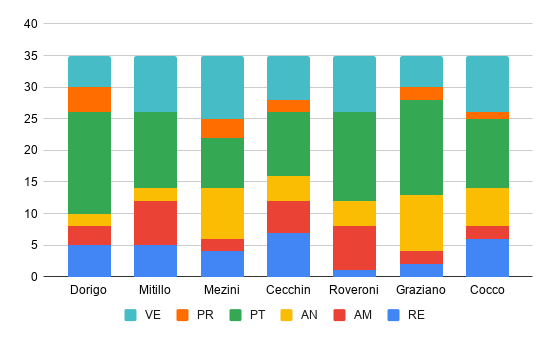
\includegraphics[width=0.7\linewidth]{../immagini/pdp/istogramma_progettazione_architetturale.png}
		\caption{Istogramma della ripartizione oraria durante la Progettazione architetturale}
	\end{center}
\end{figure}

\subsection{Prospetto economico}\label{PreventivoFaseDiProgettazioneArchitetturaleProspettoEconomico}
\quad
\def\tabularxcolumn#1{m{#1}}
{\rowcolors{2}{RawSienna!90!RawSienna!20}{RawSienna!70!RawSienna!40}
	\begin{center}
		\renewcommand{\arraystretch}{1.4}
		\begin{tabularx}{7cm}{|X|c|c|}
			\hline
			\rowcolor{airforceblue}
			\textbf{Ruolo} & \textbf{Ore} & \textbf{Costo}\\
			\hline
			Responsabile & 30 & 900\euro\\
			\hline
			Amministratore & 28 & 560\euro\\
			\hline
			Analista & 35 & 875\euro\\
			\hline
			Progettista & 86 & 1892\euro\\
			\hline
			Programmatore & 12 & 180\euro\\
			\hline
			Verificatore & 54 & 810\euro\\
			\hline
			Totale & 245 & 5217\euro\\
			\hline
		\end{tabularx}
	\captionof{table}{\textbf{Prospetto dei costi per ruolo nel periodo di Progettazione architetturale}}
	\end{center}

Il seguente grafico a torta riassume i dati ottenuti:
\begin{figure}[!ht]
	\begin{center}
		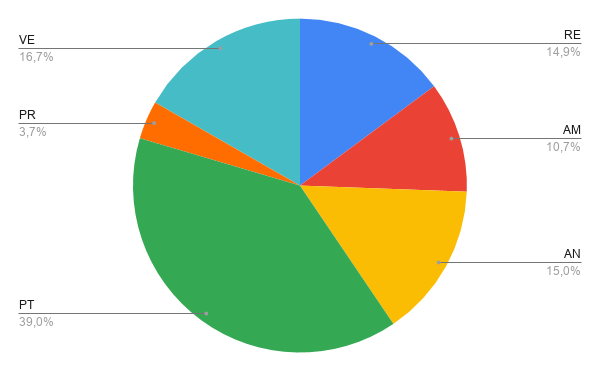
\includegraphics[width=0.8\linewidth]{../immagini/pdp/torta_progettazione_architetturale.png}
		\caption{Grafico a torta della ripartizione per ruolo delle ore nel periodo di Progettazione architetturale}
	\end{center}
\end{figure}

\section{Fase di Progettazione di dettaglio e codifica}\label{PreventivoFaseDiProgettazioneDiDettaglioECodifica}

\subsection{Primo Periodo}\label{PreventivoFaseDiProgettazioneDiDettaglioECodificaPeriodo1}

\subsubsection{Prospetto delle ore degli incrementi}\label{PreventivoFaseDiProgettazioneDiDettaglioECodificaPeriodo1Incrementi}
Di seguito riportiamo la previsione delle ore che ciascun incremento necessita, relativamente a questo periodo.
\quad
\def\tabularxcolumn#1{m{#1}}
{\rowcolors{2}{RawSienna!90!RawSienna!20}{RawSienna!70!RawSienna!40}

	\begin{center}
		\renewcommand{\arraystretch}{1.4}
		\begin{tabularx}{\textwidth}{|X|c|c|c|c|c|c|c|}
			\hline
			\rowcolor{airforceblue}
			\textbf{Incremento} & \textbf{Re} & \textbf{Am} & \textbf{An} & \textbf{Pt} & \textbf{Pr} & \textbf{Ve} & \textbf{Totale ore}\\
			\hline
			\textit{Incremento 1} & 5 & 3 & 19 & 5 & 0 & 14 & 46\\
			\hline
			\textit{Incremento 2} & 3 & 0 & 0 & 15 & 20 & 0 & 38\\
			\hline
			Totale ore ruolo & 8 & 3 & 19 & 20 & 20 & 14 & 84\\
			\hline
		\end{tabularx}
		\captionof{table}{\textbf{Prospetto delle ore degli incrementi del primo periodo della fase di Progettazione di dettaglio e codifica}}
	\end{center}

\subsubsection{Prospetto orario}\label{PreventivoFaseDiProgettazioneDiDettaglioECodificaProspettoOrarioPeriodo1}
In questa fase la distribuzione oraria è la seguente:
\quad
\def\tabularxcolumn#1{m{#1}}
{\rowcolors{2}{RawSienna!90!RawSienna!20}{RawSienna!70!RawSienna!40}

	\begin{center}
		\renewcommand{\arraystretch}{1.4}
		\begin{tabularx}{\textwidth}{|X|c|c|c|c|c|c|c|}
			\hline
			\rowcolor{airforceblue}
			\textbf{Nominativo} & \textbf{Re} & \textbf{Am} & \textbf{An} & \textbf{Pt} & \textbf{Pr} & \textbf{Ve} & \textbf{Totale ore}\\
			\hline
			\textit{Andrea Dorigo} & 3 & 0 & 3 & 4 & 2 & 1 & 13\\
			\hline
			\textit{Margherita Mitillo} & 0 & 0 & 4 & 3 & 2 & 2 & 11\\
			\hline
			\textit{Igli Mezini} & 2 & 0 & 6 & 1 & 0 & 2 & 11\\
			\hline
			\textit{Andrea Cecchin} & 0 & 3 & 0 & 4 & 5 & 2 & 14\\
			\hline
			\textit{Emma Roveroni} & 0 & 0 & 0 & 3 & 6 & 2 & 11\\
			\hline
			\textit{Alfredo Graziano} & 3 & 0 & 6 & 0 & 0 & 3 & 12\\
			\hline
			\textit{Mattia Cocco} & 0 & 0 & 0 & 5 & 5 & 2 & 12\\
			\hline
			Totale ore ruolo & 8 & 3 & 19 & 20 & 20 & 14 & 84\\
			\hline
		\end{tabularx}
	\captionof{table}{\textbf{Distribuzione delle ore del primo periodo della fase di Progettazione di dettaglio e codifica}}
	\end{center}
Il seguente istogramma riassume i dati ottenuti:
\begin{figure}[!h]
	\begin{center}
		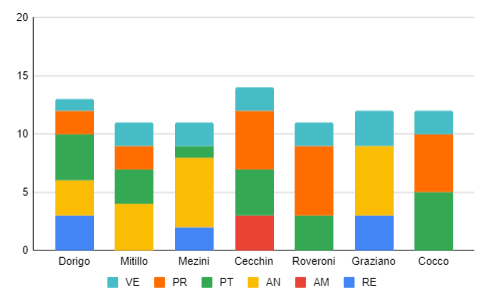
\includegraphics[width=0.7\linewidth]{../immagini/pdp/istogramma_progettazione_dettaglio_periodo1.png}
		\caption{Istogramma della ripartizione oraria durante il primo periodo della fase di Progettazione di
			dettaglio e codifica}
	\end{center}
\end{figure}
\clearpage
\subsubsection{Prospetto economico}\label{PreventivoFaseDiProgettazioneDiDettaglioECodificaProspettoEconomicoPeriodo1}
\quad
\def\tabularxcolumn#1{m{#1}}
{\rowcolors{2}{RawSienna!90!RawSienna!20}{RawSienna!70!RawSienna!40}
	\begin{center}
		\renewcommand{\arraystretch}{1.4}
		\begin{tabularx}{7cm}{|X|c|c|}
			\hline
			\rowcolor{airforceblue}
			\textbf{Ruolo} & \textbf{Ore} & \textbf{Costo}\\
			\hline
			Responsabile & 8 & 240\euro\\
			\hline
			Amministratore & 3 & 60\euro\\
			\hline
			Analista & 19 & 475\euro\\
			\hline
			Progettista & 20 & 440\euro\\
			\hline
			Programmatore & 20 & 300\euro\\
			\hline
			Verificatore & 14 & 210\euro\\
			\hline
			Totale & 84 & 1725\euro\\
			\hline
		\end{tabularx}
	\captionof{table}{\textbf{Prospetto dei costi per ruolo nel primo periodo della fase di Progettazione di dettaglio e codifica}}
	\end{center}

Il seguente grafico a torta riassume i dati ottenuti:
\begin{figure}[!ht]
	\begin{center}
		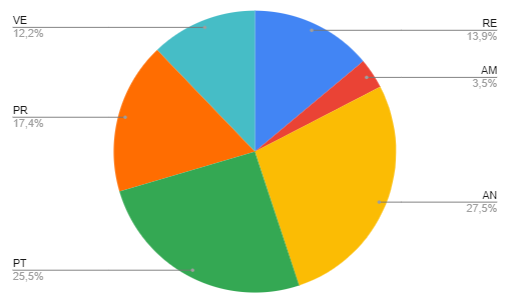
\includegraphics[width=0.8\linewidth]{../immagini/pdp/torta_progettazione_dettaglio_periodo1.png}
		\caption{Grafico a torta della ripartizione dei costi per ruolo del primo periodo della fase di Progettazione e codifica}
	\end{center}
\end{figure}

\subsection{Secondo Periodo}\label{PreventivoFaseDiProgettazioneDiDettaglioECodificaPeriodo2}

\subsubsection{Prospetto delle ore degli incrementi}\label{PreventivoFaseDiProgettazioneDiDettaglioECodificaPeriodo2Incrementi}
Di seguito riportiamo la previsione delle ore che ciascun incremento necessita, relativamente a questo periodo.
\quad
\def\tabularxcolumn#1{m{#1}}
{\rowcolors{2}{RawSienna!90!RawSienna!20}{RawSienna!70!RawSienna!40}

	\begin{center}
		\renewcommand{\arraystretch}{1.4}
		\begin{tabularx}{\textwidth}{|X|c|c|c|c|c|c|c|}
			\hline
			\rowcolor{airforceblue}
			\textbf{Incremento} & \textbf{Re} & \textbf{Am} & \textbf{An} & \textbf{Pt} & \textbf{Pr} & \textbf{Ve} & \textbf{Totale ore}\\
			\hline
			\textit{Incremento 3} & 2 & 3 & 0 & 7 & 13 & 0 & 25\\
			\hline
			\textit{Incremento 4} & 5 & 6 & 7 & 0 & 0 & 16 & 34\\
			\hline
			\textit{Incremento 5} & 2 & 4 & 0 & 11 & 18 & 0 & 35\\
			\hline
			\textit{Incremento 6} & 1 & 2 & 0 & 2 & 4 & 0 & 9\\
			\hline
			\textit{Incremento 7} & 1 & 2 & 0 & 1 & 3 & 0 & 7\\
			\hline
			\textit{Incremento 8} & 5 & 6 & 0 & 5 & 13 & 0 & 29\\
			\hline
			\textit{Incremento 9} & 6 & 7 & 0 & 13 & 0 & 16 & 42\\
			\hline
			Totale ore ruolo & 22 & 30 & 7 & 39 & 51 & 32 & 181\\
			\hline
		\end{tabularx}
		\captionof{table}{\textbf{Prospetto delle ore degli incrementi del secondo periodo della fase di Progettazione di dettaglio e codifica}}
	\end{center}

	\subsubsection{Prospetto orario}\label{PreventivoFaseDiProgettazioneDiDettaglioECodificaProspettoOrarioPeriodo2}
	In questa fase la distribuzione oraria è la seguente:
	\quad
	\def\tabularxcolumn#1{m{#1}}
	{\rowcolors{2}{RawSienna!90!RawSienna!20}{RawSienna!70!RawSienna!40}

		\begin{center}
			\renewcommand{\arraystretch}{1.4}
			\begin{tabularx}{\textwidth}{|X|c|c|c|c|c|c|c|}
				\hline
				\rowcolor{airforceblue}
				\textbf{Nominativo} & \textbf{Re} & \textbf{Am} & \textbf{An} & \textbf{Pt} & \textbf{Pr} & \textbf{Ve} & \textbf{Totale ore}\\
				\hline
				\textit{Andrea Dorigo} & 6 & 4 & 0 & 3 & 8 & 4 & 25\\
				\hline
				\textit{Margherita Mitillo} & 3 & 3 & 3 & 3 & 10 & 6 & 28\\
				\hline
				\textit{Igli Mezini} & 5 & 5 & 0 & 10 & 0 & 7 & 27\\
				\hline
				\textit{Andrea Cecchin} & 0 & 5 & 0 & 5 & 13 & 0 & 23\\
				\hline
				\textit{Emma Roveroni} & 3 & 4 & 2 & 5 & 8 & 4 & 26\\
				\hline
				\textit{Alfredo Graziano} & 5 & 6 & 0 & 8 & 0 & 7 & 26\\
				\hline
				\textit{Mattia Cocco} & 0 & 3 & 2 & 5 & 12 & 4 & 26\\
				\hline
				Totale ore ruolo & 22 & 30 & 7 & 39 & 51 & 32 & 181\\
				\hline
			\end{tabularx}
			\captionof{table}{\textbf{Distribuzione delle ore del secondo periodo della fase di Progettazione di dettaglio e codifica}}
		\end{center}
		Il seguente istogramma riassume i dati ottenuti:
		\begin{figure}[!h]
			\begin{center}
				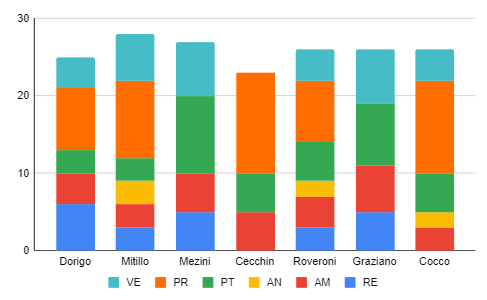
\includegraphics[width=0.7\linewidth]{../immagini/pdp/istogramma_progettazione_dettaglio_periodo2.png}
				\caption{Istogramma della ripartizione oraria durante il secondo periodo della fase di Progettazione di
					dettaglio e codifica}
			\end{center}
		\end{figure}
		\clearpage
		\subsubsection{Prospetto economico}\label{PreventivoFaseDiProgettazioneDiDettaglioECodificaProspettoEconomicoPeriodo2}
		\quad
		\def\tabularxcolumn#1{m{#1}}
		{\rowcolors{2}{RawSienna!90!RawSienna!20}{RawSienna!70!RawSienna!40}
			\begin{center}
				\renewcommand{\arraystretch}{1.4}
				\begin{tabularx}{7cm}{|X|c|c|}
					\hline
					\rowcolor{airforceblue}
					\textbf{Ruolo} & \textbf{Ore} & \textbf{Costo}\\
					\hline
					Responsabile & 22 & 660\euro\\
					\hline
					Amministratore & 30 & 600\euro\\
					\hline
					Analista & 7 & 175\euro\\
					\hline
					Progettista & 39 & 858\euro\\
					\hline
					Programmatore & 51 & 765\euro\\
					\hline
					Verificatore & 32 & 480\euro\\
					\hline
					Totale & 181 & 3538\euro\\
					\hline
				\end{tabularx}
				\captionof{table}{\textbf{Prospetto dei costi per ruolo nel secondo periodo della fase di Progettazione di dettaglio e codifica}}
			\end{center}

			Il seguente grafico a torta riassume i dati ottenuti:
			\begin{figure}[!ht]
				\begin{center}
					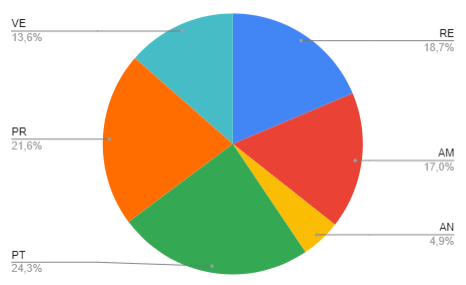
\includegraphics[width=0.8\linewidth]{../immagini/pdp/torta_progettazione_dettaglio_periodo2.png}
					\caption{Grafico a torta della ripartizione dei costi per ruolo del secondo periodo della fase di Progettazione e codifica}
				\end{center}
			\end{figure}

\subsection{Terzo Periodo}\label{PreventivoFaseDiProgettazioneDiDettaglioECodificaPeriodo3}

\subsubsection{Prospetto delle ore degli incrementi}\label{PreventivoFaseDiProgettazioneDiDettaglioECodificaPeriodo3Incrementi}
Di seguito riportiamo la previsione delle ore che ciascun incremento necessita, relativamente a questo periodo.
\quad
\def\tabularxcolumn#1{m{#1}}
{\rowcolors{2}{RawSienna!90!RawSienna!20}{RawSienna!70!RawSienna!40}

	\begin{center}
		\renewcommand{\arraystretch}{1.4}
		\begin{tabularx}{\textwidth}{|X|c|c|c|c|c|c|c|}
			\hline
			\rowcolor{airforceblue}
			\textbf{Incremento} & \textbf{Re} & \textbf{Am} & \textbf{An} & \textbf{Pt} & \textbf{Pr} & \textbf{Ve} & \textbf{Totale ore}\\
			\hline
			\textit{Incremento 10} & 3 & 3 & 0 & 8 & 0 & 30 & 44\\
			\hline
			\textit{Incremento 11} & 2 & 2 & 0 & 2 & 0 & 0 & 6\\
			\hline
			Totale ore ruolo & 5 & 5 & 0 & 10 & 0 & 30 & 50\\
			\hline
		\end{tabularx}
		\captionof{table}{\textbf{Prospetto delle ore degli incrementi del terzo periodo della fase di Progettazione di dettaglio e codifica}}
	\end{center}

	\subsubsection{Prospetto orario}\label{PreventivoFaseDiProgettazioneDiDettaglioECodificaProspettoOrarioPeriodo3}
	In questa fase la distribuzione oraria è la seguente:
	\quad
	\def\tabularxcolumn#1{m{#1}}
	{\rowcolors{2}{RawSienna!90!RawSienna!20}{RawSienna!70!RawSienna!40}

		\begin{center}
			\renewcommand{\arraystretch}{1.4}
			\begin{tabularx}{\textwidth}{|X|c|c|c|c|c|c|c|}
				\hline
				\rowcolor{airforceblue}
				\textbf{Nominativo} & \textbf{Re} & \textbf{Am} & \textbf{An} & \textbf{Pt} & \textbf{Pr} & \textbf{Ve} & \textbf{Totale ore}\\
				\hline
				\textit{Andrea Dorigo} & 2 & 0 & 0 & 0 & 0 & 5 & 7\\
				\hline
				\textit{Margherita Mitillo} & 0 & 1 & 0 & 2 & 0 & 3 & 6\\
				\hline
				\textit{Igli Mezini} & 2 & 0 & 0 & 3 & 0 & 2 & 7\\
				\hline
				\textit{Andrea Cecchin} & 0 & 2 & 0 & 0 & 0 & 6 & 8\\
				\hline
				\textit{Emma Roveroni} & 0 & 1 & 0 & 2 & 0 & 5 & 8\\
				\hline
				\textit{Alfredo Graziano} & 1 & 0 & 0 & 3 & 0 & 3 & 7\\
				\hline
				\textit{Mattia Cocco} & 0 & 1 & 0 & 0 & 0 & 6 & 7\\
				\hline
				Totale ore ruolo & 5 & 5 & 0 & 10 & 0 & 30 & 50\\
				\hline
			\end{tabularx}
			\captionof{table}{\textbf{Distribuzione delle ore del terzo periodo della fase di Progettazione di dettaglio e codifica}}
		\end{center}
		Il seguente istogramma riassume i dati ottenuti:
		\begin{figure}[!h]
			\begin{center}
				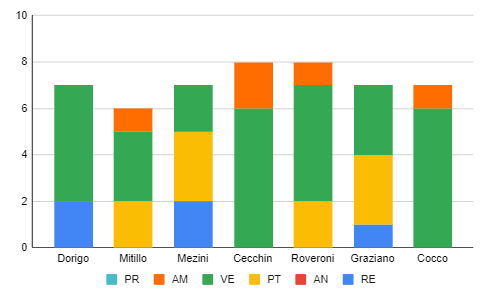
\includegraphics[width=0.7\linewidth]{../immagini/pdp/istogramma_progettazione_dettaglio_periodo3.png}
				\caption{Istogramma della ripartizione oraria durante il terzo periodo della fase di Progettazione di
					dettaglio e codifica}
			\end{center}
		\end{figure}
		\clearpage
		\subsubsection{Prospetto economico}\label{PreventivoFaseDiProgettazioneDiDettaglioECodificaProspettoEconomicoPeriodo3}
		\quad
		\def\tabularxcolumn#1{m{#1}}
		{\rowcolors{2}{RawSienna!90!RawSienna!20}{RawSienna!70!RawSienna!40}
			\begin{center}
				\renewcommand{\arraystretch}{1.4}
				\begin{tabularx}{7cm}{|X|c|c|}
					\hline
					\rowcolor{airforceblue}
					\textbf{Ruolo} & \textbf{Ore} & \textbf{Costo}\\
					\hline
					Responsabile & 5 & 150\euro\\
					\hline
					Amministratore & 5 & 100\euro\\
					\hline
					Analista & 0 & 0\euro\\
					\hline
					Progettista & 10 & 220\euro\\
					\hline
					Programmatore & 0 & 0\euro\\
					\hline
					Verificatore & 30 & 450\euro\\
					\hline
					Totale & 50 & 920\euro\\
					\hline
				\end{tabularx}
				\captionof{table}{\textbf{Prospetto dei costi per ruolo nel terzo periodo della fase di Progettazione di dettaglio e codifica}}
			\end{center}

			Il seguente grafico a torta riassume i dati ottenuti:
			\begin{figure}[!ht]
				\begin{center}
					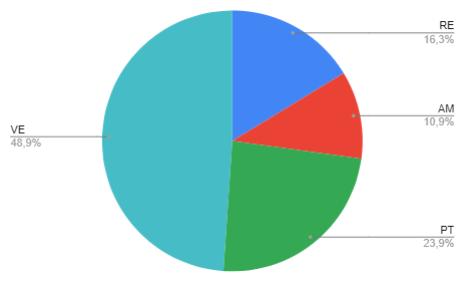
\includegraphics[width=0.8\linewidth]{../immagini/pdp/torta_progettazione_dettaglio_periodo3.png}
					\caption{Grafico a torta della ripartizione dei costi per ruolo del terzo periodo della fase di Progettazione e codifica}
				\end{center}
			\end{figure}

		\subsection{Prospetto complessivo}\label{PreventivoFaseDiProgettazioneDiDettaglioECodificaComplessivo}

			\subsubsection{Prospetto orario}\label{PreventivoFaseDiProgettazioneDiDettaglioECodificaProspettoOrario}
			In questa fase la distribuzione oraria è la seguente:
			\quad
			\def\tabularxcolumn#1{m{#1}}
			{\rowcolors{2}{RawSienna!90!RawSienna!20}{RawSienna!70!RawSienna!40}

				\begin{center}
					\renewcommand{\arraystretch}{1.4}
					\begin{tabularx}{\textwidth}{|X|c|c|c|c|c|c|c|}
						\hline
						\rowcolor{airforceblue}
						\textbf{Nominativo} & \textbf{Re} & \textbf{Am} & \textbf{An} & \textbf{Pt} & \textbf{Pr} & \textbf{Ve} & \textbf{Totale ore}\\
						\hline
						\textit{Andrea Dorigo} & 11 & 4 & 3 & 7 & 10 & 10 & 45\\
						\hline
						\textit{Margherita Mitillo} & 3 & 4 & 7 & 8 & 12 & 11 & 45\\
						\hline
						\textit{Igli Mezini} & 9 & 5 & 6 & 14 & 0 & 11 & 45\\
						\hline
						\textit{Andrea Cecchin} & 0 & 10 & 0 & 9 & 18 & 8 & 45\\
						\hline
						\textit{Emma Roveroni} & 3 & 5 & 2 & 10 & 14 & 11 & 45\\
						\hline
						\textit{Alfredo Graziano} & 9 & 6 & 6 & 11 & 0 & 13 & 45\\
						\hline
						\textit{Mattia Cocco} & 0 & 4 & 2 & 10 & 17 & 12 & 45\\
						\hline
						Totale ore ruolo & 35 & 38 & 26 & 69 & 71 & 76 & 315\\
						\hline
					\end{tabularx}
					\captionof{table}{\textbf{Distribuzione delle ore durante la Progettazione di dettaglio e codifica}}
				\end{center}
				Il seguente istogramma riassume i dati ottenuti:
				\begin{figure}[!h]
					\begin{center}
						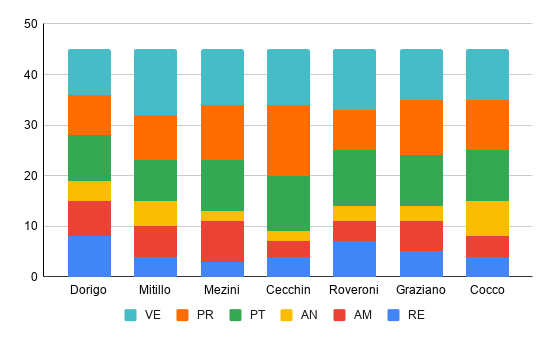
\includegraphics[width=0.7\linewidth]{../immagini/pdp/istogramma_progettazione_dettaglio.png}
						\caption{Istogramma della ripartizione oraria durante la Progettazione di
							dettaglio e codifica}
					\end{center}
				\end{figure}
				\clearpage
				\subsubsection{Prospetto economico}\label{PreventivoFaseDiProgettazioneDiDettaglioECodificaProspettoEconomico}
				\quad
				\def\tabularxcolumn#1{m{#1}}
				{\rowcolors{2}{RawSienna!90!RawSienna!20}{RawSienna!70!RawSienna!40}
					\begin{center}
						\renewcommand{\arraystretch}{1.4}
						\begin{tabularx}{7cm}{|X|c|c|}
							\hline
							\rowcolor{airforceblue}
							\textbf{Ruolo} & \textbf{Ore} & \textbf{Costo}\\
							\hline
							Responsabile & 35 & 1050\euro\\
							\hline
							Amministratore & 38 & 760\euro\\
							\hline
							Analista & 26 & 650\euro\\
							\hline
							Progettista & 69 & 1518\euro\\
							\hline
							Programmatore & 71 & 1065\euro\\
							\hline
							Verificatore & 76 & 1140\euro\\
							\hline
							Totale & 315 & 6183\euro\\
							\hline
						\end{tabularx}
						\captionof{table}{\textbf{Prospetto dei costi per ruolo nel periodo di Progettazione di dettaglio e codifica}}
					\end{center}

					Il seguente grafico a torta riassume i dati ottenuti:
					\begin{figure}[!ht]
						\begin{center}
							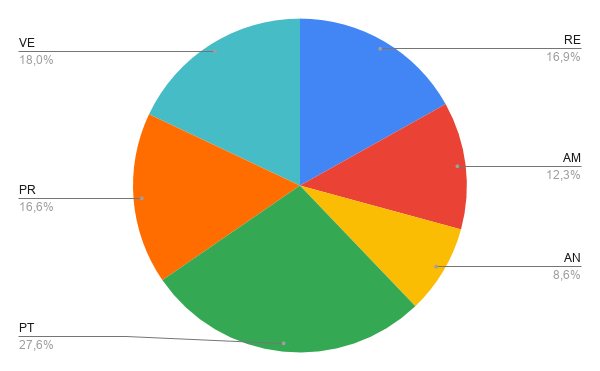
\includegraphics[width=0.8\linewidth]{../immagini/pdp/torta_progettazione_dettaglio.png}
							\caption{Grafico a torta della ripartizione dei costi per ruolo nella fase di Progettazione
								di dettaglio e codifica}
						\end{center}
					\end{figure}

\section{Fase di Validazione e collaudo}\label{PreventivoFaseDiProgettazionediValidazioneECollaudo}

% \subsection{Primo periodo}\label{PreventivoFaseDiProgettazionediValidazioneECollaudoPrimoPeriodo}
\subsection{Prospetto delle ore degli incrementi 12, 13 e 14}\label{PreventivoFaseDiProgettazionediValidazioneECollaudoIncrementi12-13-14}
Di seguito riportiamo la previsione delle ore che ciascun incremento necessita, relativamente agli incrementi 12, 13 e 14.
\quad
\def\tabularxcolumn#1{m{#1}}
{\rowcolors{2}{RawSienna!90!RawSienna!20}{RawSienna!70!RawSienna!40}

	\begin{center}
		\renewcommand{\arraystretch}{1.4}
		\begin{tabularx}{\textwidth}{|X|c|c|c|c|c|c|c|}
			\hline
			\rowcolor{airforceblue}
			\textbf{Incremento} & \textbf{Re} & \textbf{Am} & \textbf{An} & \textbf{Pt} & \textbf{Pr} & \textbf{Ve} & \textbf{Totale ore}\\
			\hline
			\textit{Incremento 12} & 2 & 3 & 0 & 0 & 14 & 0 & 19\\
			\hline
			\textit{Incremento 13} & 1 & 2 & 0 & 0 & 0 & 10 & 13\\
			\hline
			\textit{Incremento 14} & 2 & 3 & 0 & 0 & 0 & 13 & 18\\
			\hline
			Totale ore ruolo & 5 & 8 & 0 & 0 & 14 & 23 & 50\\
			\hline
		\end{tabularx}
		\captionof{table}{\textbf{Prospetto delle ore degli incrementi 12, 13 e 14 della fase di Validazione e Collaudo}}
	\end{center}

\subsubsection{Prospetto orario}\label{PreventivoFaseDiProgettazionediValidazioneECollaudoIncrementi12-13-14ProspettoOrario}
Per questi tre incrementi la distribuzione oraria tra i componenti del gruppo sarà la seguente:

\quad
\def\tabularxcolumn#1{m{#1}}
{\rowcolors{2}{RawSienna!90!RawSienna!20}{RawSienna!70!RawSienna!40}

	\begin{center}
		\renewcommand{\arraystretch}{1.4}
		\begin{tabularx}{\textwidth}{|X|c|c|c|c|c|c|c|}
			\hline
			\rowcolor{airforceblue}
			\textbf{Nominativo} & \textbf{Re} & \textbf{Am} & \textbf{An} & \textbf{Pt} & \textbf{Pr} & \textbf{Ve} & \textbf{Totale ore}\\
			\hline
			\textit{Andrea Dorigo} & 2 & 0 & 0 & 0 & 0 & 6 & 8\\
			\hline
			\textit{Margherita Mitillo} & 0 & 3 & 0 & 0 & 2 & 3 & 8\\
			\hline
			\textit{Igli Mezini} & 2 & 0 & 0 & 0 & 2 & 2 & 6\\
			\hline
			\textit{Andrea Cecchin} & 0 & 3 & 0 & 0 & 2 & 3 & 8\\
			\hline
			\textit{Emma Roveroni} & 0 & 2 & 0 & 0 & 2 & 3 & 7\\
			\hline
			\textit{Alfredo Graziano} & 1 & 0 & 0 & 0 & 2 & 3 & 6\\
			\hline
			\textit{Mattia Cocco} & 0 & 0 & 0 & 0 & 4 & 3 & 7\\
			\hline
			Totale ore ruolo & 5 & 8 & 0 & 0 & 14 & 23 & 50\\
			\hline
		\end{tabularx}
		\captionof{table}{\textbf{Distribuzione oraria degli incrementi 12, 13 e 14 della fase di Validazione e Collaudo}}
	\end{center}

Il seguente istogramma riassume i dati ottenuti:
\begin{figure}[!h]
	\begin{center}
		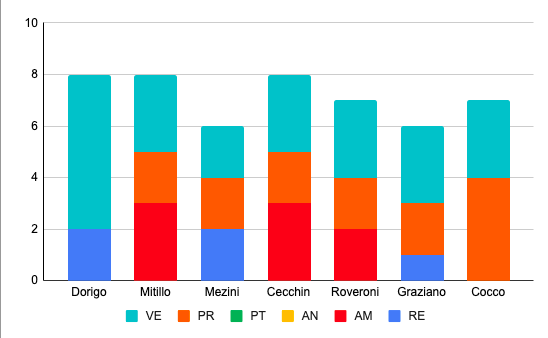
\includegraphics[width=0.7\linewidth]{../immagini/pdp/istogramma_validazione_collaudo_periodo1.png}
		\caption{Istogramma della ripartizione oraria durante gli incrementi 12, 13 e 14 della fase di Validazione e Collaudo}
	\end{center}
\end{figure}
\clearpage

\subsubsection{Prospetto economico}\label{PreventivoFaseDiProgettazionediValidazioneECollaudoIncrementi12-13-14ProspettoEconomico}
\quad
\def\tabularxcolumn#1{m{#1}}
{\rowcolors{2}{RawSienna!90!RawSienna!20}{RawSienna!70!RawSienna!40}
	\begin{center}
		\renewcommand{\arraystretch}{1.4}
		\begin{tabularx}{7cm}{|X|c|c|}
			\hline
			\rowcolor{airforceblue}
			\textbf{Ruolo} & \textbf{Ore} & \textbf{Costo}\\
			\hline
			Responsabile & 5 & 150\euro\\
			\hline
			Amministratore & 8 & 160\euro\\
			\hline
			Analista & 0 & 0\euro\\
			\hline
			Progettista & 0 & 0\euro\\
			\hline
			Programmatore & 14 & 210\euro\\
			\hline
			Verificatore & 23 & 345\euro\\
			\hline
			Totale & 50 & 865\euro\\
			\hline
		\end{tabularx}
		\captionof{table}{\textbf{Prospetto dei costi per ruolo per gli incrementi 12, 13 e 14 della fase di Validazione e collaudo}}
	\end{center}

	Il seguente grafico a torta riassume i dati ottenuti:
	\begin{figure}[!ht]
		\begin{center}
			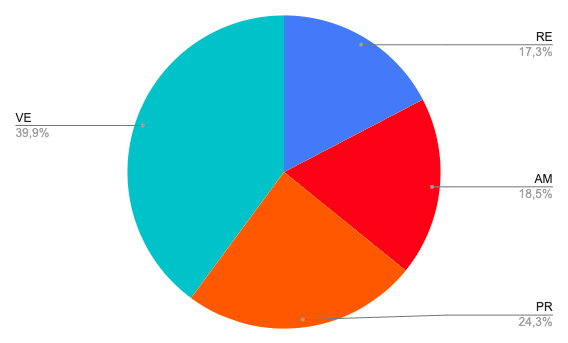
\includegraphics[width=0.8\linewidth]{../immagini/pdp/torta_validazione_collaudo_periodo1.png}
			\caption{Grafico a torta della ripartizione dei costi per ruolo del per gli incrementi 12, 13 e 14 della fase di Validazione e Collaudo}
		\end{center}
	\end{figure}

% \subsection{Secondo periodo}\label{PreventivoFaseDiProgettazionediValidazioneECollaudoSecondoPeriodo}
\subsection{Prospetto delle ore degli incrementi 15 e 16}\label{PreventivoFaseDiProgettazionediValidazioneECollaudoIncrementi15-16}
Di seguito riportiamo la previsione delle ore che ciascun incremento necessita, relativamente agli incrementi 15 e 16.
\quad
\def\tabularxcolumn#1{m{#1}}
{\rowcolors{2}{RawSienna!90!RawSienna!20}{RawSienna!70!RawSienna!40}

	\begin{center}
		\renewcommand{\arraystretch}{1.4}
		\begin{tabularx}{\textwidth}{|X|c|c|c|c|c|c|c|}
			\hline
			\rowcolor{airforceblue}
			\textbf{Incremento} & \textbf{Re} & \textbf{Am} & \textbf{An} & \textbf{Pt} & \textbf{Pr} & \textbf{Ve} & \textbf{Totale ore}\\
			\hline
			\textit{Incremento 15} & 3 & 7 & 0 & 0 & 24 & 0 & 34\\
			\hline
			\textit{Incremento 16} & 8 & 6 & 0 & 0 & 0 & 37 & 51\\
			\hline
			Totale ore ruolo & 11 & 13 & 0 & 0 & 24 & 37 & 85\\
			\hline
		\end{tabularx}
		\captionof{table}{\textbf{Prospetto delle ore degli incrementi degli intervalli 15 e 16 della fase di Validazione e Collaudo}}
	\end{center}

	\subsubsection{Prospetto orario}\label{PreventivoFaseDiProgettazionediValidazioneECollaudoIncrementi15-16ProspettoOrario}
	Per gli incrementi 15 e 16 la distribuzione oraria tra i componenti del gruppo sarà la seguente:

	\quad
	\def\tabularxcolumn#1{m{#1}}
	{\rowcolors{2}{RawSienna!90!RawSienna!20}{RawSienna!70!RawSienna!40}

		\begin{center}
			\renewcommand{\arraystretch}{1.4}
			\begin{tabularx}{\textwidth}{|X|c|c|c|c|c|c|c|}
				\hline
				\rowcolor{airforceblue}
				\textbf{Nominativo} & \textbf{Re} & \textbf{Am} & \textbf{An} & \textbf{Pt} & \textbf{Pr} & \textbf{Ve} & \textbf{Totale ore}\\
				\hline
				\textit{Andrea Dorigo} & 3 & 1 & 0 & 0 & 3 & 4 & 11\\
				\hline
				\textit{Margherita Mitillo} & 1 & 3 & 0 & 0 & 2 & 6 & 12\\
				\hline
				\textit{Igli Mezini} & 2 & 3 & 0 & 0 & 3 & 7 & 15\\
				\hline
				\textit{Andrea Cecchin} & 0 & 2 & 0 & 0 & 5 & 5 & 12\\
				\hline
				\textit{Emma Roveroni} & 2 & 0 & 0 & 0 & 4 & 4 & 10\\
				\hline
				\textit{Alfredo Graziano} & 3 & 2 & 0 & 0 & 3 & 7 & 15\\
				\hline
				\textit{Mattia Cocco} & 0 & 2 & 0 & 0 & 4 & 4 & 10\\
				\hline
				Totale ore ruolo & 11 & 13 & 0 & 0 & 24 & 37 & 85\\
				\hline
			\end{tabularx}
			\captionof{table}{\textbf{Distribuzione oraria degli incrementi 15 e 16 della fase di Validazione e Collaudo}}
		\end{center}

		Il seguente istogramma riassume i dati ottenuti:
		\begin{figure}[!h]
			\begin{center}
				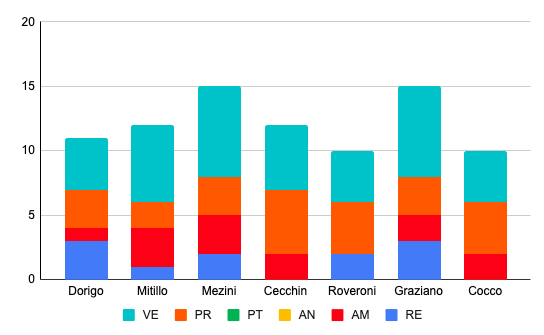
\includegraphics[width=0.7\linewidth]{../immagini/pdp/istogramma_validazione_collaudo_periodo2.png}
				\caption{Istogramma della ripartizione oraria durante gli incrementi 15 e 16 della fase di Validazione e Collaudo}
			\end{center}
		\end{figure}
		\clearpage

		\subsubsection{Prospetto economico}\label{PreventivoFaseDiProgettazionediValidazioneECollaudoIncrementi15-16ProspettoEconomico}
		\quad
		\def\tabularxcolumn#1{m{#1}}
		{\rowcolors{2}{RawSienna!90!RawSienna!20}{RawSienna!70!RawSienna!40}
			\begin{center}
				\renewcommand{\arraystretch}{1.4}
				\begin{tabularx}{7cm}{|X|c|c|}
					\hline
					\rowcolor{airforceblue}
					\textbf{Ruolo} & \textbf{Ore} & \textbf{Costo}\\
					\hline
					Responsabile & 11 & 330\euro\\
					\hline
					Amministratore & 13 & 260\euro\\
					\hline
					Analista & 0 & 0\euro\\
					\hline
					Progettista & 0 & 0\euro\\
					\hline
					Programmatore & 24 & 360\euro\\
					\hline
					Verificatore & 37 & 555\euro\\
					\hline
					Totale & 85 & 1505\euro\\
					\hline
				\end{tabularx}
				\captionof{table}{\textbf{Prospetto dei costi per ruolo degli incrementi 15 e 16 della fase di Validazione e collaudo}}
			\end{center}

			Il seguente grafico a torta riassume i dati ottenuti:
			\begin{figure}[!ht]
				\begin{center}
					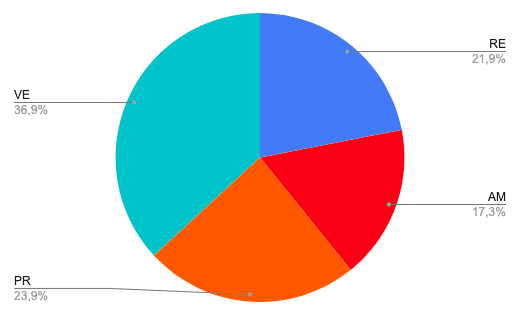
\includegraphics[width=0.8\linewidth]{../immagini/pdp/torta_validazione_collaudo_periodo2.png}
					\caption{Grafico a torta della ripartizione dei costi per ruolo degli incrementi 15 e 16 della fase di Validazione e Collaudo}
				\end{center}
			\end{figure}

% \subsection{Terzo periodo}\label{PreventivoFaseDiProgettazionediValidazioneECollaudoTerzoPeriodo}
\subsection{Prospetto delle ore degli incrementi 17 e 18}\label{PreventivoFaseDiProgettazionediValidazioneECollaudoIncrementi17-18}
Di seguito riportiamo la previsione delle ore che gli incrementi 17 e 18 necessitano:
\quad
\def\tabularxcolumn#1{m{#1}}
{\rowcolors{2}{RawSienna!90!RawSienna!20}{RawSienna!70!RawSienna!40}

	\begin{center}
		\renewcommand{\arraystretch}{1.4}
		\begin{tabularx}{\textwidth}{|X|c|c|c|c|c|c|c|}
			\hline
			\rowcolor{airforceblue}
			\textbf{Incremento} & \textbf{Re} & \textbf{Am} & \textbf{An} & \textbf{Pt} & \textbf{Pr} & \textbf{Ve} & \textbf{Totale ore}\\
			\hline
			\textit{Incremento 17} & 3 & 2 & 0 & 0 & 14 & 0 & 19\\
			\hline
			\textit{Incremento 18} & 2 & 5 & 0 & 0 & 14 & 0 & 21\\
			\hline
			Totale ore ruolo & 5 & 7 & 0 & 0 & 28 & 0 & 40\\
			\hline
		\end{tabularx}
		\captionof{table}{\textbf{Prospetto delle ore degli incrementi 17 e 18 della fase di Validazione e Collaudo}}
	\end{center}

	\subsubsection{Prospetto orario}\label{PreventivoFaseDiProgettazionediValidazioneECollaudoIncrementi17-18ProspettoOrario}
	Per questi incrementi la distribuzione oraria tra i componenti del gruppo sarà la seguente:

	\quad
	\def\tabularxcolumn#1{m{#1}}
	{\rowcolors{2}{RawSienna!90!RawSienna!20}{RawSienna!70!RawSienna!40}

		\begin{center}
			\renewcommand{\arraystretch}{1.4}
			\begin{tabularx}{\textwidth}{|X|c|c|c|c|c|c|c|}
				\hline
				\rowcolor{airforceblue}
				\textbf{Nominativo} & \textbf{Re} & \textbf{Am} & \textbf{An} & \textbf{Pt} & \textbf{Pr} & \textbf{Ve} & \textbf{Totale ore}\\
				\hline
				\textit{Andrea Dorigo} & 2 & 0 & 0 & 0 & 4 & 0 & 6\\
				\hline
				\textit{Margherita Mitillo} & 0 & 2 & 0 & 0 & 3 & 0 & 5\\
				\hline
				\textit{Igli Mezini} & 2 & 0 & 0 & 0 & 2 & 0 & 4\\
				\hline
				\textit{Andrea Cecchin} & 0 & 2 & 0 & 0 & 3 & 0 & 5\\
				\hline
				\textit{Emma Roveroni} & 0 & 1 & 0 & 0 & 7 & 0 & 8\\
				\hline
				\textit{Alfredo Graziano} & 1 & 0 & 0 & 0 & 3 & 0 & 4\\
				\hline
				\textit{Mattia Cocco} & 0 & 2 & 0 & 0 & 6 & 0 & 8\\
				\hline
				Totale ore ruolo & 5 & 7 & 0 & 0 & 28 & 0 & 40\\
				\hline
			\end{tabularx}
			\captionof{table}{\textbf{Distribuzione oraria degli incrementi 17 e 18 della fase di Validazione e Collaudo}}
		\end{center}

		Il seguente istogramma riassume i dati ottenuti:
		\begin{figure}[!h]
			\begin{center}
				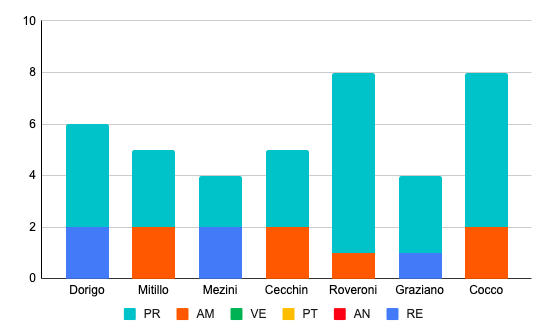
\includegraphics[width=0.7\linewidth]{../immagini/pdp/istogramma_validazione_collaudo_periodo3.png}
				\caption{Istogramma della ripartizione oraria durante gli incrementi 17 e 18 della fase di Validazione e Collaudo}
			\end{center}
		\end{figure}
		\clearpage

		\subsubsection{Prospetto economico}\label{PreventivoFaseDiProgettazionediValidazioneECollaudoIncrmenti17-18ProspettoEconomico}
		\quad
		\def\tabularxcolumn#1{m{#1}}
		{\rowcolors{2}{RawSienna!90!RawSienna!20}{RawSienna!70!RawSienna!40}
			\begin{center}
				\renewcommand{\arraystretch}{1.4}
				\begin{tabularx}{7cm}{|X|c|c|}
					\hline
					\rowcolor{airforceblue}
					\textbf{Ruolo} & \textbf{Ore} & \textbf{Costo}\\
					\hline
					Responsabile & 5 & 150\euro\\
					\hline
					Amministratore & 7 & 140\euro\\
					\hline
					Analista & 0 & 0\euro\\
					\hline
					Progettista & 0 & 0\euro\\
					\hline
					Programmatore & 28 & 420\euro\\
					\hline
					Verificatore & 0 & 0\euro\\
					\hline
					Totale & 40 & 710\euro\\
					\hline
				\end{tabularx}
				\captionof{table}{\textbf{Prospetto dei costi per ruolo negli incrementi 17 e 18 della fase di Validazione e collaudo}}
			\end{center}

			Il seguente grafico a torta riassume i dati ottenuti:
			\begin{figure}[!ht]
				\begin{center}
					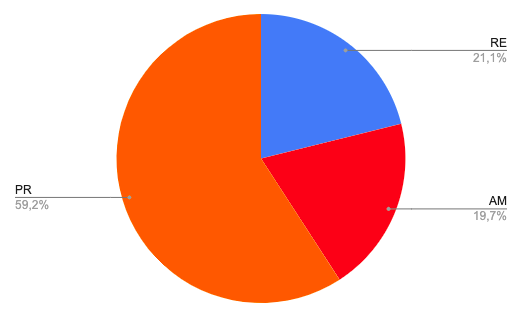
\includegraphics[width=0.8\linewidth]{../immagini/pdp/torta_validazione_collaudo_periodo3.png}
					\caption{Grafico a torta della ripartizione dei costi per ruolo degli incrementi 17 e 18 della fase di Validazione e Collaudo}
				\end{center}
			\end{figure}

\subsection{Prospetto complessivo}\label{PreventivoFaseValidazioneCollaudoComplessivo}
\subsubsection{Prospetto orario}\label{PreventivoFaseValidazioneCollaudoComplessivoProspettoOrario}
La distribuzione oraria totale di questa fase è la seguente:
\quad
\def\tabularxcolumn#1{m{#1}}
{\rowcolors{2}{RawSienna!90!RawSienna!20}{RawSienna!70!RawSienna!40}

	\begin{center}
		\renewcommand{\arraystretch}{1.4}
		\begin{tabularx}{\textwidth}{|X|c|c|c|c|c|c|c|}
			\hline
			\rowcolor{airforceblue}
			\textbf{Nominativo} & \textbf{Re} & \textbf{Am} & \textbf{An} & \textbf{Pt} & \textbf{Pr} & \textbf{Ve} & \textbf{Totale ore}\\
			\hline
			\textit{Andrea Dorigo} & 7 & 1 & 0 & 0 & 7 & 10 & 25\\
			\hline
			\textit{Margherita Mitillo} & 1 & 8 & 0 & 0 & 7 & 9 & 25\\
			\hline
			\textit{Igli Mezini} & 6 & 3 & 0 & 0 & 7 & 9 & 25\\
			\hline
			\textit{Andrea Cecchin} & 0 & 7 & 0 & 0 & 10 & 8 & 25\\
			\hline
			\textit{Emma Roveroni} & 2 & 3 & 0 & 0 & 13 & 7 & 25\\
			\hline
			\textit{Alfredo Graziano} & 5 & 2 & 0 & 0 & 8 & 10 & 25\\
			\hline
			\textit{Mattia Cocco} & 0 & 4 & 0 & 0 & 14 & 7 & 25\\
			\hline
			Totale ore ruolo & 21 & 28 & 0 & 0 & 66 & 60 & 175\\
			\hline
		\end{tabularx}
	\captionof{table}{\textbf{Distribuzione delle ore totali durante la fase di Validazione e collaudo}}
	\end{center}
Il seguente istogramma riassume i dati ottenuti:
\begin{figure}[!ht]
	\begin{center}
		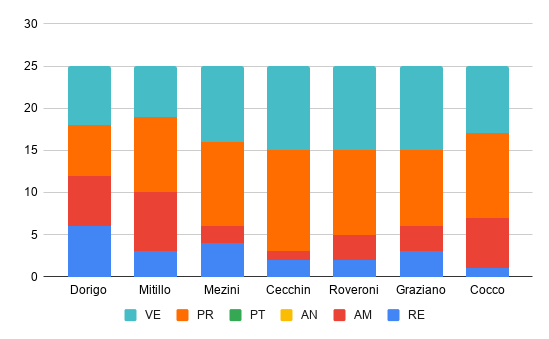
\includegraphics[width=0.7\linewidth]{../immagini/pdp/istogramma_validazione.png}
		\caption{Istogramma della ripartizione oraria durante la fase di Validazione e
			collaudo}
	\end{center}
\end{figure}
\clearpage
\subsubsection{Prospetto economico}\label{PreventivoFaseValidazioneCollaudoComplessivooProspettoEconomico}
\quad
\def\tabularxcolumn#1{m{#1}}
{\rowcolors{2}{RawSienna!90!RawSienna!20}{RawSienna!70!RawSienna!40}
	\begin{center}
		\renewcommand{\arraystretch}{1.4}
		\begin{tabularx}{7cm}{|X|c|c|}
			\hline
			\rowcolor{airforceblue}
			\textbf{Ruolo} & \textbf{Ore} & \textbf{Costo}\\
			\hline
			Responsabile & 21 & 630\euro\\
			\hline
			Amministratore & 28 & 560\euro\\
			\hline
			Analista & 0 & 0\euro\\
			\hline
			Progettista & 0 & 0\euro\\
			\hline
			Programmatore & 66 & 990\euro\\
			\hline
			Verificatore & 60 & 900\euro\\
			\hline
			Totale & 175 & 3080\euro\\
			\hline
		\end{tabularx}
	\captionof{table}{\textbf{Prospetto dei costi per ruolo nella fase di Validazione e collaudo}}
	\end{center}

Il seguente grafico a torta riassume i dati ottenuti:
\begin{figure}[!ht]
	\begin{center}
		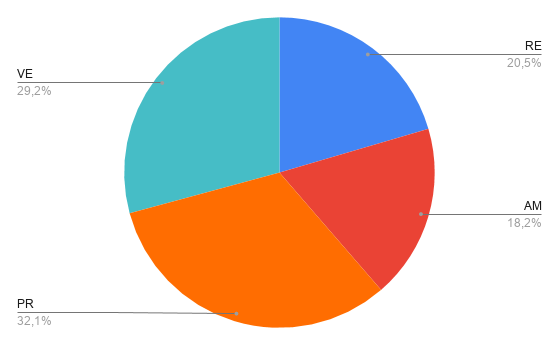
\includegraphics[width=0.8\linewidth]{../immagini/pdp/torta_validazione.png}
		\caption{Grafico a torta della ripartizione dei costi per ruolo della fase di Validazione e Collaudo}
	\end{center}
\end{figure}

\section{Riepilogo}\label{PreventivoRiepilogo}

\subsection{Ore totali}\label{PreventivoRiepilogoOreTotali}

\subsubsection{Suddivisione lavoro}\label{PreventivoRiepilogoOreTotaliSuddivisioneDelLavoro}
Nella seguente tabella vengono riportate il totale delle ore del progetto, sono presenti sia le ore di investimento, sia quelle rendicontate a carico del committente$_G$.
\quad
\def\tabularxcolumn#1{m{#1}}
{\rowcolors{2}{RawSienna!90!RawSienna!20}{RawSienna!70!RawSienna!40}

	\begin{center}
		\renewcommand{\arraystretch}{1.4}
		\begin{tabularx}{\textwidth}{|X|c|c|c|c|c|c|c|}
			\hline
			\rowcolor{airforceblue}
			\textbf{Nominativo} & \textbf{Re} & \textbf{Am} & \textbf{An} & \textbf{Pt} & \textbf{Pr} & \textbf{Ve} & \textbf{Totale ore}\\
			\hline
			\textit{Andrea Dorigo} & 33 & 17 & 8 & 23 & 21 & 32 & 134\\
			\hline
			\textit{Margherita Mitillo} & 17 & 24 & 23 & 20 & 19 & 31 & 134\\
			\hline
			\textit{Igli Mezini} & 23 & 17 & 22 & 22 & 10 & 40 & 134\\
			\hline
			\textit{Andrea Cecchin} & 13 & 31 & 15 & 19 & 30 & 26 & 134\\
			\hline
			\textit{Emma Roveroni} & 9 & 21 & 13 & 24 & 27 & 40 & 134\\
			\hline
			\textit{Alfredo Graziano} & 17 & 22 & 25 & 26 & 10 & 34 & 134\\
			\hline
			\textit{Mattia Cocco} & 8 & 19 & 17 & 21 & 32 & 37 & 134\\
			\hline
		\end{tabularx}
	\captionof{table}{\textbf{Distribuzione delle ore totali di investimento e rendicontate}}
	\end{center}

Il seguente istogramma riassume i dati ottenuti:
\begin{figure}[!h]
	\begin{center}
		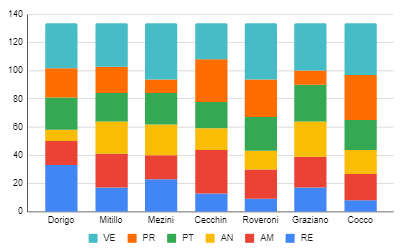
\includegraphics[width=0.65\linewidth]{../immagini/pdp/istogramma_suddivisione_lavoro1.png}
		\caption{Istogramma della ripartizione oraria totali di investimento e rendicontate}
	\end{center}
\end{figure}

\subsubsection{Prospetto economico}\label{PreventivoRiepilogoOreTotaliProspettoEconomico}
I costi da affrontare per ogni ruolo sono:
\quad
\def\tabularxcolumn#1{m{#1}}
{\rowcolors{2}{RawSienna!90!RawSienna!20}{RawSienna!70!RawSienna!40}
	\begin{center}
		\renewcommand{\arraystretch}{1.4}
		\begin{tabularx}{7cm}{|X|c|c|}
			\hline
			\rowcolor{airforceblue}
			\textbf{Ruolo} & \textbf{Ore} & \textbf{Costo}\\
			\hline
			Responsabile & 118 & 3540\euro\\
			\hline
			Amministratore & 153 & 3060\euro\\
			\hline
			Analista & 123 & 3075\euro\\
			\hline
			Progettista & 155 & 3410\euro\\
			\hline
			Programmatore & 149 & 2235\euro\\
			\hline
			Verificatore & 240 & 3600\euro\\
			\hline
			Totale & 938 & 18920\euro\\
			\hline
		\end{tabularx}
	\captionof{table}{\textbf{Prospetto dei costi totali delle ore totali di investimento e rendicontate}}
	\end{center}

Il seguente grafico a torta riassume i dati ottenuti:
\begin{figure}[!ht]
	\begin{center}
		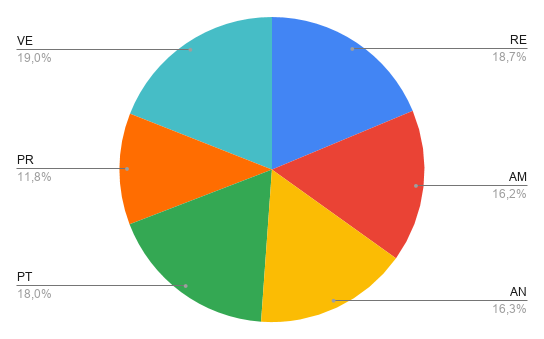
\includegraphics[width=0.8\linewidth]{../immagini/pdp/torta_suddvisione_lavoro.png}
		\caption{Grafico a torta della ripartizione dei costi per ruolo totali di investimento e
			rendicontate}
	\end{center}
\end{figure}

\subsection{Ore rendicontate}\label{PreventivoRiepilogoOreRendicontate}

\subsubsection{Suddivisione lavoro}\label{PreventivoRiepilogoOreRendicontateSuddivisioneLavoro}
Le ore rendicontate sono riportate nella seguente tabella:
\quad
\def\tabularxcolumn#1{m{#1}}
{\rowcolors{2}{RawSienna!90!RawSienna!20}{RawSienna!70!RawSienna!40}

	\begin{center}
		\renewcommand{\arraystretch}{1.4}
		\begin{tabularx}{\textwidth}{|X|c|c|c|c|c|c|c|}
			\hline
			\rowcolor{airforceblue}
			\textbf{Nominativo} & \textbf{Re} & \textbf{Am} & \textbf{An} & \textbf{Pt} & \textbf{Pr} & \textbf{Ve} & \textbf{Totale ore}\\
			\hline
			\textit{Andrea Dorigo} & 23 & 8 & 5 & 23 & 21 & 25 & 105\\
			\hline
			\textit{Margherita Mitillo} & 9 & 19 & 9 & 20 & 19 & 29 & 105\\
			\hline
			\textit{Igli Mezini} & 19 & 10 & 14 & 22 & 10 & 30 & 105\\
			\hline
			\textit{Andrea Cecchin} & 7 & 22 & 4 & 19 & 30 & 23 & 105\\
			\hline
			\textit{Emma Roveroni} & 6 & 15 & 6 & 24 & 27 & 27 & 105\\
			\hline
			\textit{Alfredo Graziano} & 16 & 10 & 15 & 26 & 10 & 28 & 105\\
			\hline
			\textit{Mattia Cocco} & 6 & 10 & 8 & 21 & 32 & 28 & 105\\
			\hline
		\end{tabularx}
	\captionof{table}{\textbf{Distribuzione delle ore rendicontate}}
	\end{center}
Il seguente istogramma riassume i dati ottenuti:
\begin{figure}[!ht]
	\begin{center}
		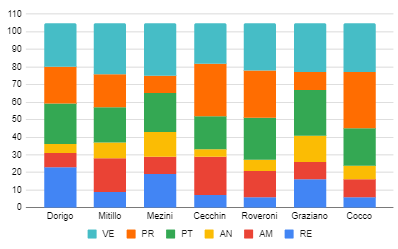
\includegraphics[width=0.8\linewidth]{../immagini/pdp/istogramma_rendicontate1.png}
		\caption{Istogramma della ripartizione oraria rendicontate}
	\end{center}
\end{figure}

\subsubsection{Prospetto economico}\label{PreventivoRiepilogoOreRendicontateProspettoEconomico}
Il totale rendicontato dei costi da affrontare per ogni ruolo è il seguenti:
\quad
\def\tabularxcolumn#1{m{#1}}
{\rowcolors{2}{RawSienna!90!RawSienna!20}{RawSienna!70!RawSienna!40}
	\begin{center}
		\renewcommand{\arraystretch}{1.4}
		\begin{tabularx}{7cm}{|X|c|c|}
			\hline
			\rowcolor{airforceblue}
			\textbf{Ruolo} & \textbf{Ore} & \textbf{Costo}\\
			\hline
			Responsabile & 86 & 2580\euro\\
			\hline
			Amministratore & 94 & 1880\euro\\
			\hline
			Analista & 61 & 1525\euro\\
			\hline
			Progettista & 155 & 3410\euro\\
			\hline
			Programmatore & 149 & 2235\euro\\
			\hline
			Verificatore & 190 & 2850\euro\\
			\hline
			Totale & 735 & 14480\euro\\
			\hline
		\end{tabularx}
	\captionof{table}{\textbf{Prospetto dei costi totali delle ore rendicontate}}
	\end{center}
Il seguente grafico a torta riassume i dati ottenuti:
\begin{figure}[!ht]
	\begin{center}
		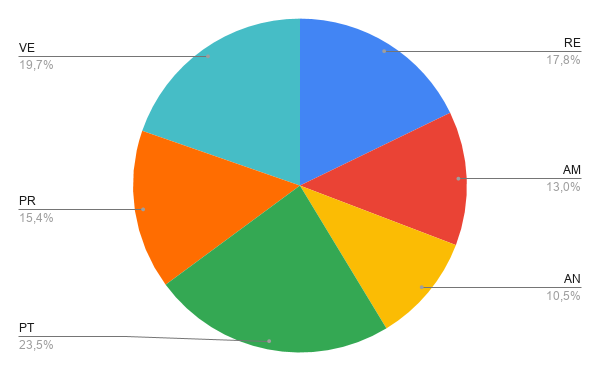
\includegraphics[width=0.8\linewidth]{../immagini/pdp/torta_rendicontate.png}
		\caption{Grafico a torta della ripartizione per ruolo delle ore rendicontate}
	\end{center}
\end{figure}
\subsection{Conclusioni}\label{PreventivoRiepilogoConclusioni}
Il costo totale del progetto considerando solamente le ore rendicontate è: 14480\euro.
